\section{What Can a Target Read Resolve?}
\subsection{The command seen by the receiving controller}
Let $x_t^\star$ and $x_t$ denote the demonstrated and replayed hand positions just before command $t$. The source command specifies a translation $a_t$ in metres after action scaling, and writes the target $g_t^\star$. The recorded hand need not have reached that target. We score the hand against the recorded hand at the same post-step time and score the target separately at the instant it is written.

Let $b_t$ be the command origin, $s$ the per-axis limits, and $C$ the workspace clip. A legal displacement $d$ writes
\begin{equation}
 F(b_t,d)=C(b_t+d),\quad -s\le d\le s .\label{eq:setter}
\end{equation}
Fetch uses the measured gripper position as $b_t$. Sawyer uses its last written target. On the source tape, Fetch's hand and command determine $g_t^\star$. On Sawyer the initial target and the commands applied during the clean demonstration determine it recursively. A replay read supplies the current \emph{destination} origin. It leaves the source tape unchanged.

To retain the lag between hand and target in the demonstration, we request $h_t=g_t^\star+k(x_t^\star-x_t)$, where $k$ is the hand feedback gain. For an origin estimate $b$, project $h_t$ onto the reachable box $[C(b-s),C(b+s)]$ to obtain $q$. Sending $d=\operatorname{clip}_{[-s,s]}(q-b)$ realizes $q$ if $b$ is the true origin and the command reaches the setter.

\subsection{A tight error floor for two compatible histories}
Suppose the observations and sent commands leave two possible origins, $b$ and $b-v$. For example, a hidden overwrite could replace $v$ by zero. Take $h=b$ and assume the workspace is locally inactive and $v$ is an admissible displacement. Sending a common $d$ incurs Euclidean errors $\|d\|_2$ and $\|d-v\|_2$. By the triangle inequality their larger value is at least $\|v\|_2/2$, attained by $d=v/2$. A program that insists on zero error for the first history must send $d=0$ and incur $\|v\|_2$ on the other. An exact read allows a different command in each history and zero error on both. The ambiguity lasts only as long as both histories remain compatible with the available observations.

We tested this construction on Sawyer's native setter at 16 reset states across push and drawer-open. We held the hand, joint positions and joint velocities fixed, separated the stored origins along one axis by 2, 5 or 8\,mm, and issued zero, midpoint and exact corrections. Across 144 matched problems (864 writes), the largest absolute difference from the predicted residual was below $10^{-10}$\,mm (Fig.~\ref{fig:ambiguity}).
\begin{figure}[t]
\centering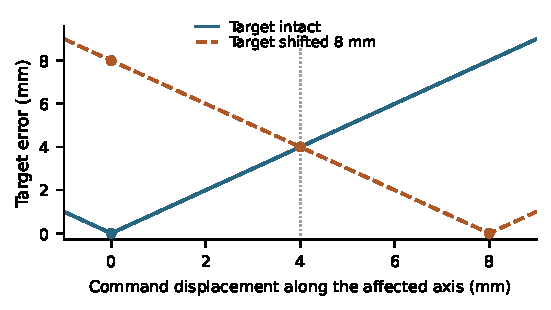
\includegraphics[width=\columnwidth]{figures/ambiguity.pdf}
\caption{One native Sawyer setter state with two origins 8\,mm apart. Lines show the predicted write errors for a shared displacement on one axis. The dots show native setter writes. A 4\,mm midpoint gives the smallest worst error without a read. Reading the origin lets the program choose the zero-error action for each history.}\label{fig:ambiguity}
\end{figure}
